%%%%%%%%%%%%%%%%%%%%%%%%%%%%%%%%%%%%%%%%%
% Beamer Presentation
% LaTeX Template
% Version 1.0 (10/11/12)
%
% This template has been downloaded from:
% http://www.LaTeXTemplates.com
%
% License:
% CC BY-NC-SA 3.0 (http://creativecommons.org/licenses/by-nc-sa/3.0/)
%
%%%%%%%%%%%%%%%%%%%%%%%%%%%%%%%%%%%%%%%%%

%----------------------------------------------------------------------------------------
%	PACKAGES AND THEMES
%----------------------------------------------------------------------------------------

\documentclass{beamer}
\usepackage[french]{babel}
\usepackage[utf8x]{inputenc}

\mode<presentation> {

% The Beamer class comes with a number of default slide themes
% which change the colors and layouts of slides. Below this is a list
% of all the themes, uncomment each in turn to see what they look like.

%\usetheme{default}
%\usetheme{AnnArbor}
%\usetheme{Antibes}
%\usetheme{Bergen}
%\usetheme{Berkeley}
%\usetheme{Berlin}
%\usetheme{Boadilla}
\usetheme{CambridgeUS}
%\usetheme{Copenhagen}
%\usetheme{Darmstadt}
%\usetheme{Dresden}
%\usetheme{Frankfurt}
%\usetheme{Goettingen}
%\usetheme{Hannover}
%\usetheme{Ilmenau}
%\usetheme{JuanLesPins}
%\usetheme{Luebeck}
%\usetheme{Madrid}
%\usetheme{Malmoe}
%\usetheme{Marburg}
%\usetheme{Montpellier}
%\usetheme{PaloAlto}
%\usetheme{Pittsburgh}
%\usetheme{Rochester}
%\usetheme{Singapore}
%\usetheme{Szeged}
%\usetheme{Warsaw}

% As well as themes, the Beamer class has a number of color themes
% for any slide theme. Uncomment each of these in turn to see how it
% changes the colors of your current slide theme.

%\usecolortheme{albatross}
\usecolortheme{beaver}
%\usecolortheme{beetle}
%\usecolortheme{crane}
%\usecolortheme{dolphin}
%\usecolortheme{dove}
%\usecolortheme{fly}
%\usecolortheme{lily}
%\usecolortheme{orchid}
%\usecolortheme{rose}
%\usecolortheme{seagull}
%\usecolortheme{seahorse}
%\usecolortheme{whale}
%\usecolortheme{wolverine}

%\setbeamertemplate{footline} % To remove the footer line in all slides uncomment this line
%\setbeamertemplate{footline}[page number] % To replace the footer line in all slides with a simple slide count uncomment this line

\setbeamertemplate{navigation symbols}{} % To remove the navigation symbols from the bottom of all slides uncomment this line

\setbeamertemplate{headline}{} % To remove headline uncomment this line
}

\usepackage{graphicx} % Allows including images
\usepackage{booktabs} % Allows the use of \toprule, \midrule and \bottomrule in tables

%----------------------------------------------------------------------------------------
%	TITLE PAGE
%----------------------------------------------------------------------------------------

\title[Soutenance PSAR]{Application embarquée sur carte pour l'automobile} % The short title appears at the bottom of every slide, the full title is only on the title page

\author{M. Bittan, R. Gouicem, I. Toumlilt} % Your name
\institute[UPMC] % Your institution as it will appear on the bottom of every slide, may be shorthand to save space
{
UPMC \\ % Your institution for the title page
\medskip
\textit{Encadrants: A. Blin, G. Muller, J. Sopena} % Your email address
}
\date{11 mai 2015} % Date, can be changed to a custom date

\titlegraphic{
  
\includegraphics[height=0.6cm]{include/logo_upmc.png}%  % Include a department/university logo - this will require the graphicx package
  \hspace{1cm}%
  
\includegraphics[height=0.9cm]{include/logo_lip6.png}% % Include a department/university logo - this will require the graphicx package
  \hspace{1cm}%
  
\includegraphics[height=0.9cm]{include/logo_renault.png}}


\begin{document}

\begin{frame}
\titlepage % Print the title page as the first slide
\end{frame}

\begin{frame}
\frametitle{Contexte}
\begin{itemize}
  \item Automobile = système distribué
    \vspace{1em}
  \item Exécution de tâches à criticités mixtes
    \begin{itemize}
      \item Tâches \textit{best-effort}: GPS, infotainment
      \item Tâches \textit{temps-réel}: ABS, airbag, régulateur de distance
    \end{itemize}
    \vspace{1em}
  \item Assurer la sécurité et la fiabilité du système
\end{itemize}
\end{frame}

%---------------------------------------------------------

\begin{frame}
  \frametitle{Contexte (2)}
  \visible<1->{
    \only<1>{
      \begin{center}
        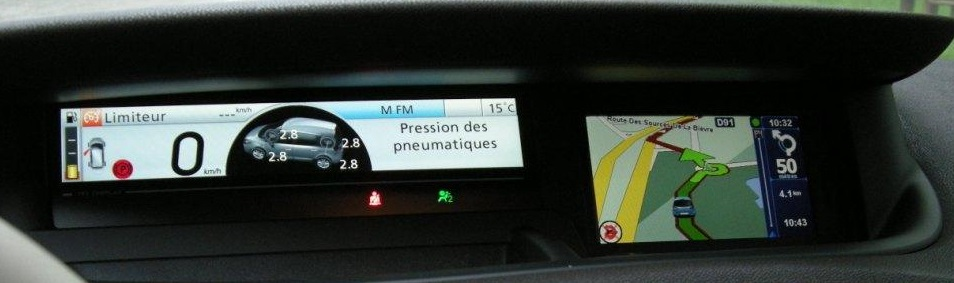
\includegraphics[scale=0.7]{include/tableau_de_bord1.jpg}
      \end{center}
    }
    \only<2->{
      \begin{center}
        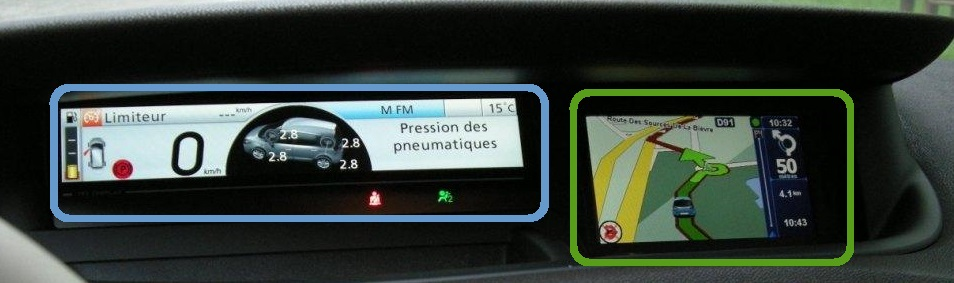
\includegraphics[scale=0.7]{include/tableau_de_bord2.jpg}
      \end{center}
    }
  }
  \visible<3->{
    \begin{center}
      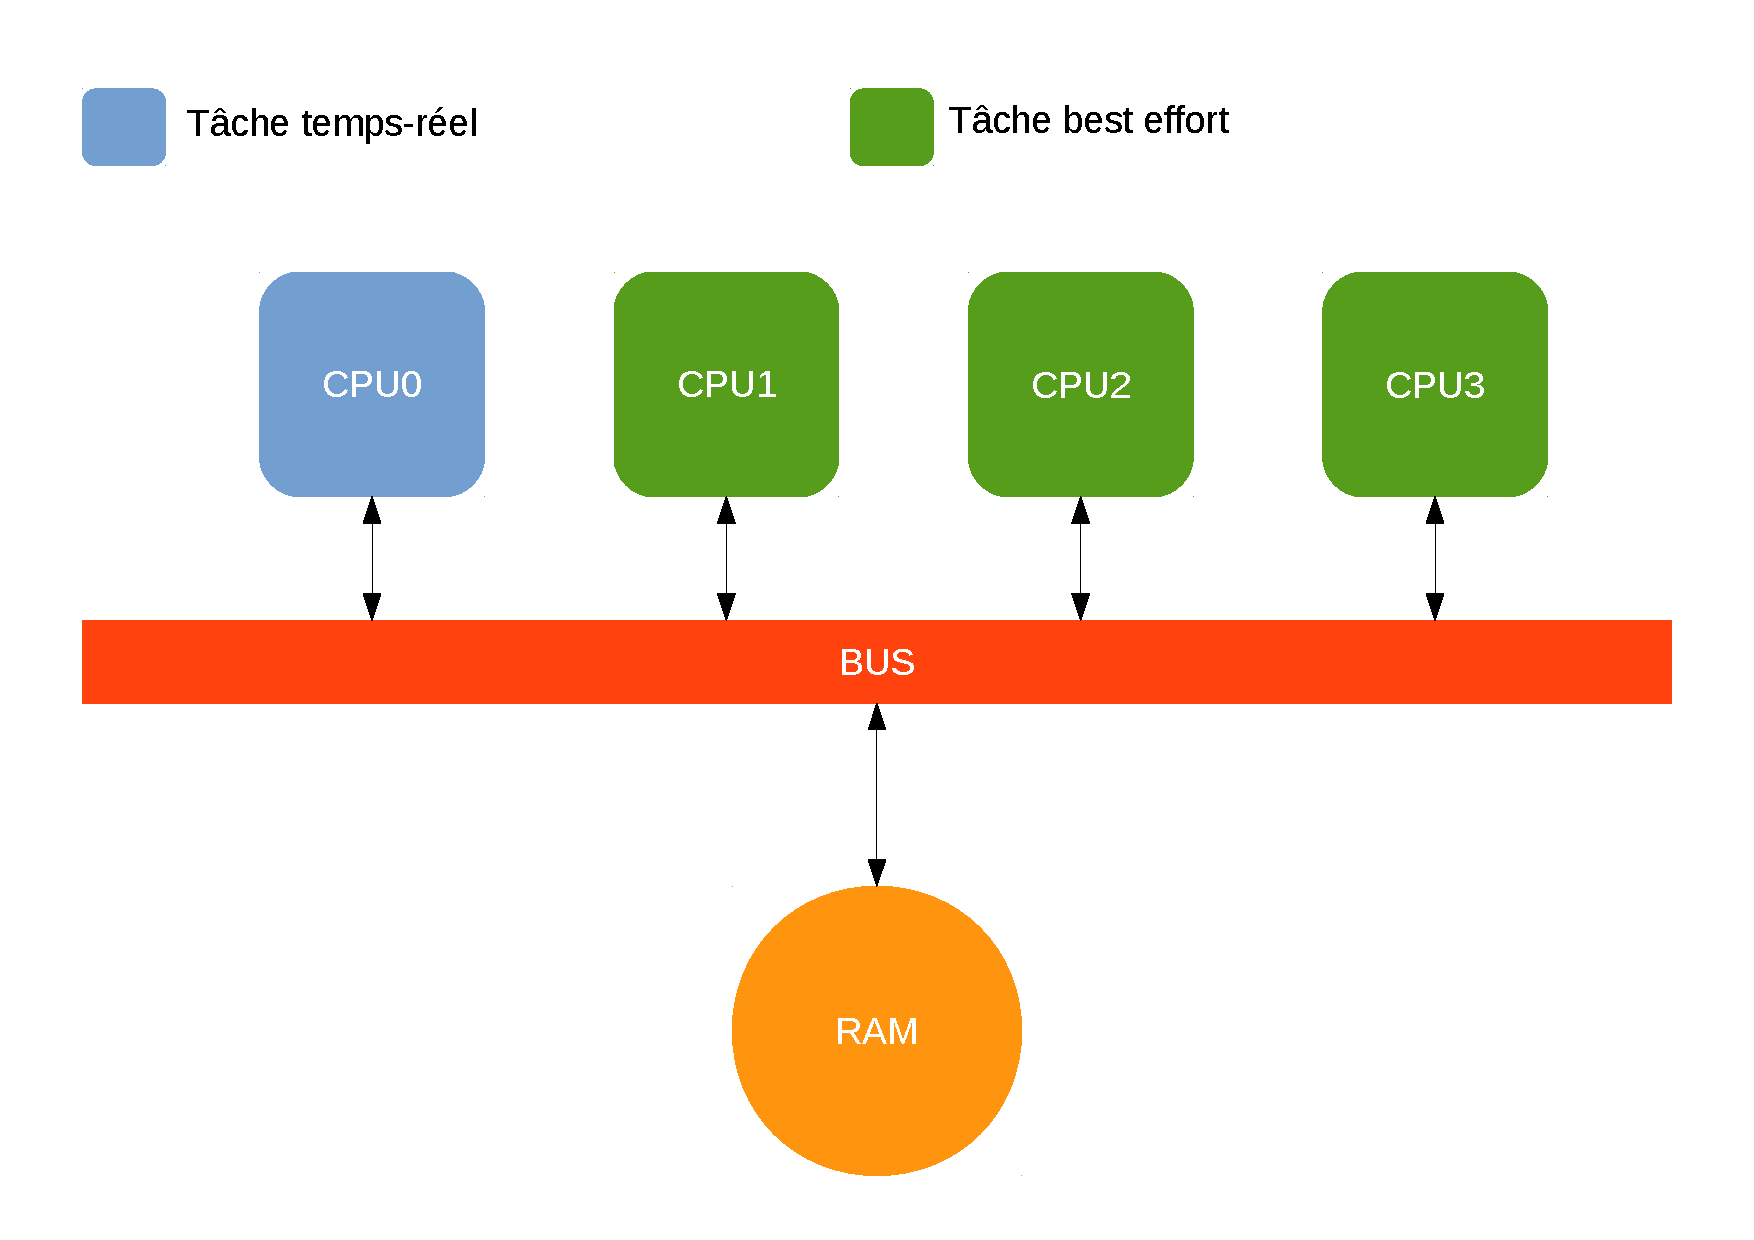
\includegraphics[trim=0 0 0 130,clip,scale=0.2]{include/archi.pdf}
    \end{center}
  }
  \visible<4>{
    \begin{alertblock}{Problèmes}
      Gestion du partage des ressources, et notamment du bus.
    \end{alertblock}
  }
\end{frame}

\begin{frame}
  \frametitle{Objectifs}
  Placé dans le cadre de la thèse d'Antoine Blin en cours au Lip6, ce projet SAR
  a pour objectifs :
  \vspace{1em}
  \begin{enumerate}
  \item Le choix d'une application pour automobile à fort trafic mémoire
    \vspace{1em}
  \item Le portage de cette application sur la carte embarquée
    \vspace{1em}
  \item La parallélisation de cette application
    \vspace{1em}
  \item L'étude de l'impact de cette application sur une tâche temps-réel
  \end{enumerate}
\end{frame}

\begin{frame}
  \frametitle{Choix de l'application}
  \framesubtitle{Critères de sélection}
  \begin{block}{Type d'application}
    Nous avons choisi de porter une application de calcul d'itinéraires car elles
    manipulent des graphes de tailles importantes.
  \end{block}
  Les autres critères sont :
  \begin{itemize}
  \item Langage : pas de \textit{JVM}
    \vspace{1em}
  \item Consommation mémoire contenue : 1 Go de RAM sur la carte
    \vspace{1em}
  \item Nombre de dépendances faible
    \vspace{1em}
  \item Parallélisable
  \end{itemize}
\end{frame}

\begin{frame}
  \frametitle{Choix de l'application}
  \framesubtitle{Comparaison des candidats}
  \begin{block}{}
    Deux applications, écrites en C++ et C, se sont dégagées :
  \end{block}
  \begin{tabular}{c|c}
    \textbf{Open Street Routing Machine} & \textbf{Routino} \\
    \hline
    \visible<2->{
      \begin{minipage}{5cm}
        \vspace{1em}
        \begin{itemize}
        \item[$+$] Parallèle (client-serveur)
          \vspace{1em}
        \item[$-$] Nombre de dépendances
          \vspace{1em}
        \item[$-$] Trop gourmand en mémoire
        \end{itemize}
      \end{minipage}
    }
    &
    \visible<3->{
      \begin{minipage}{5cm}
        \vspace{1em}
        \begin{itemize}
        \item[$+$] Aucune dépendance
          \vspace{1em}
        \item[$+$] Peu gourmand en mémoire
          \vspace{1em}
        \item[$-$] Pas parallèle
        \end{itemize}
      \end{minipage}
    }
  \end{tabular}
  \visible<4->{
    \begin{exampleblock}{Application choisie}
      Routino pour sa facilité de portage et son occupation mémoire contenue.
    \end{exampleblock}
  }
\end{frame}



%----------------------------------------------------

\begin{frame}
  \frametitle{Parallélisation de Routino}
  \framesubtitle{Deux approches possibles}
  \begin{itemize}
  \item Parallélisation de l'algorithme
    \begin{itemize}
    \item Trop de dépendances de données
    \item Trop de points de synchronisation
    \end{itemize}
    \vspace{1em}
  \item Parallélisation par segments
    \begin{itemize}
    \item Prédécouper l'itinéraire en segments
    \item Calculer chaque segment séparément
    \end{itemize}
  \end{itemize}
\end{frame}

% --------------------------------------------------

\begin{frame}
  \frametitle{Parallélisation de Routino}
  \framesubtitle{Approche par segments}
  \begin{columns}[t]
    \visible<1->{
      \begin{column}{0.5\textwidth}
        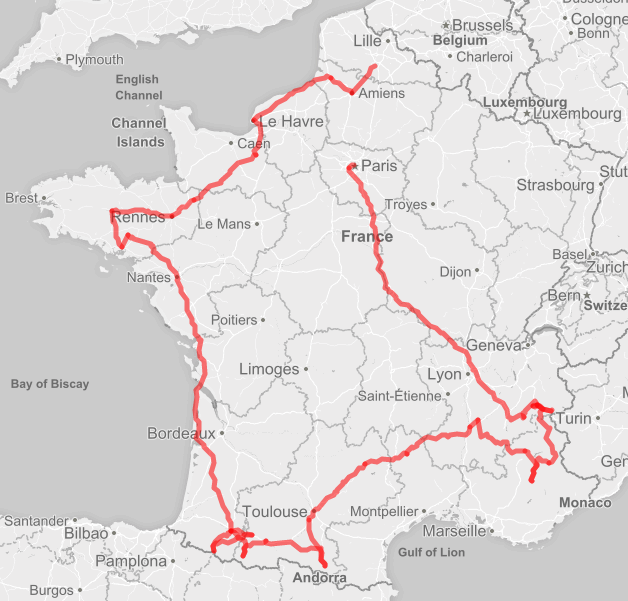
\includegraphics[scale=0.25]{include/tourfrance_mono.png}
      \end{column}
    }
    \visible<2->{
      \begin{column}{0.5\textwidth}
        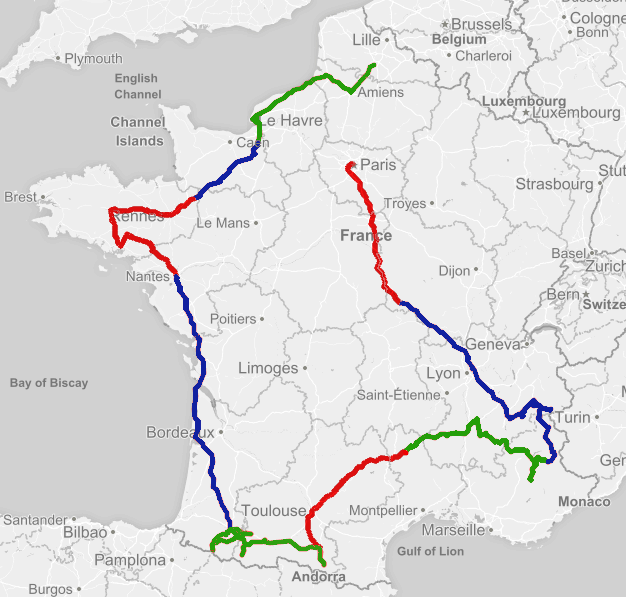
\includegraphics[scale=0.25]{include/tourfrance_multi.png}
      \end{column}
    }
  \end{columns}
  \visible<3->{
    \begin{alertblock}{Difficulté d'implantation}
      Les segments doivent être indépendants et le nombre de points de
      synchronisation faible.
    \end{alertblock}
  }
\end{frame}

% --------------------------------------------------

\begin{frame}
  \frametitle{Parallélisation de Routino}
  \framesubtitle{Déroulement de l'exécution}
  \begin{center}
    \only<1>{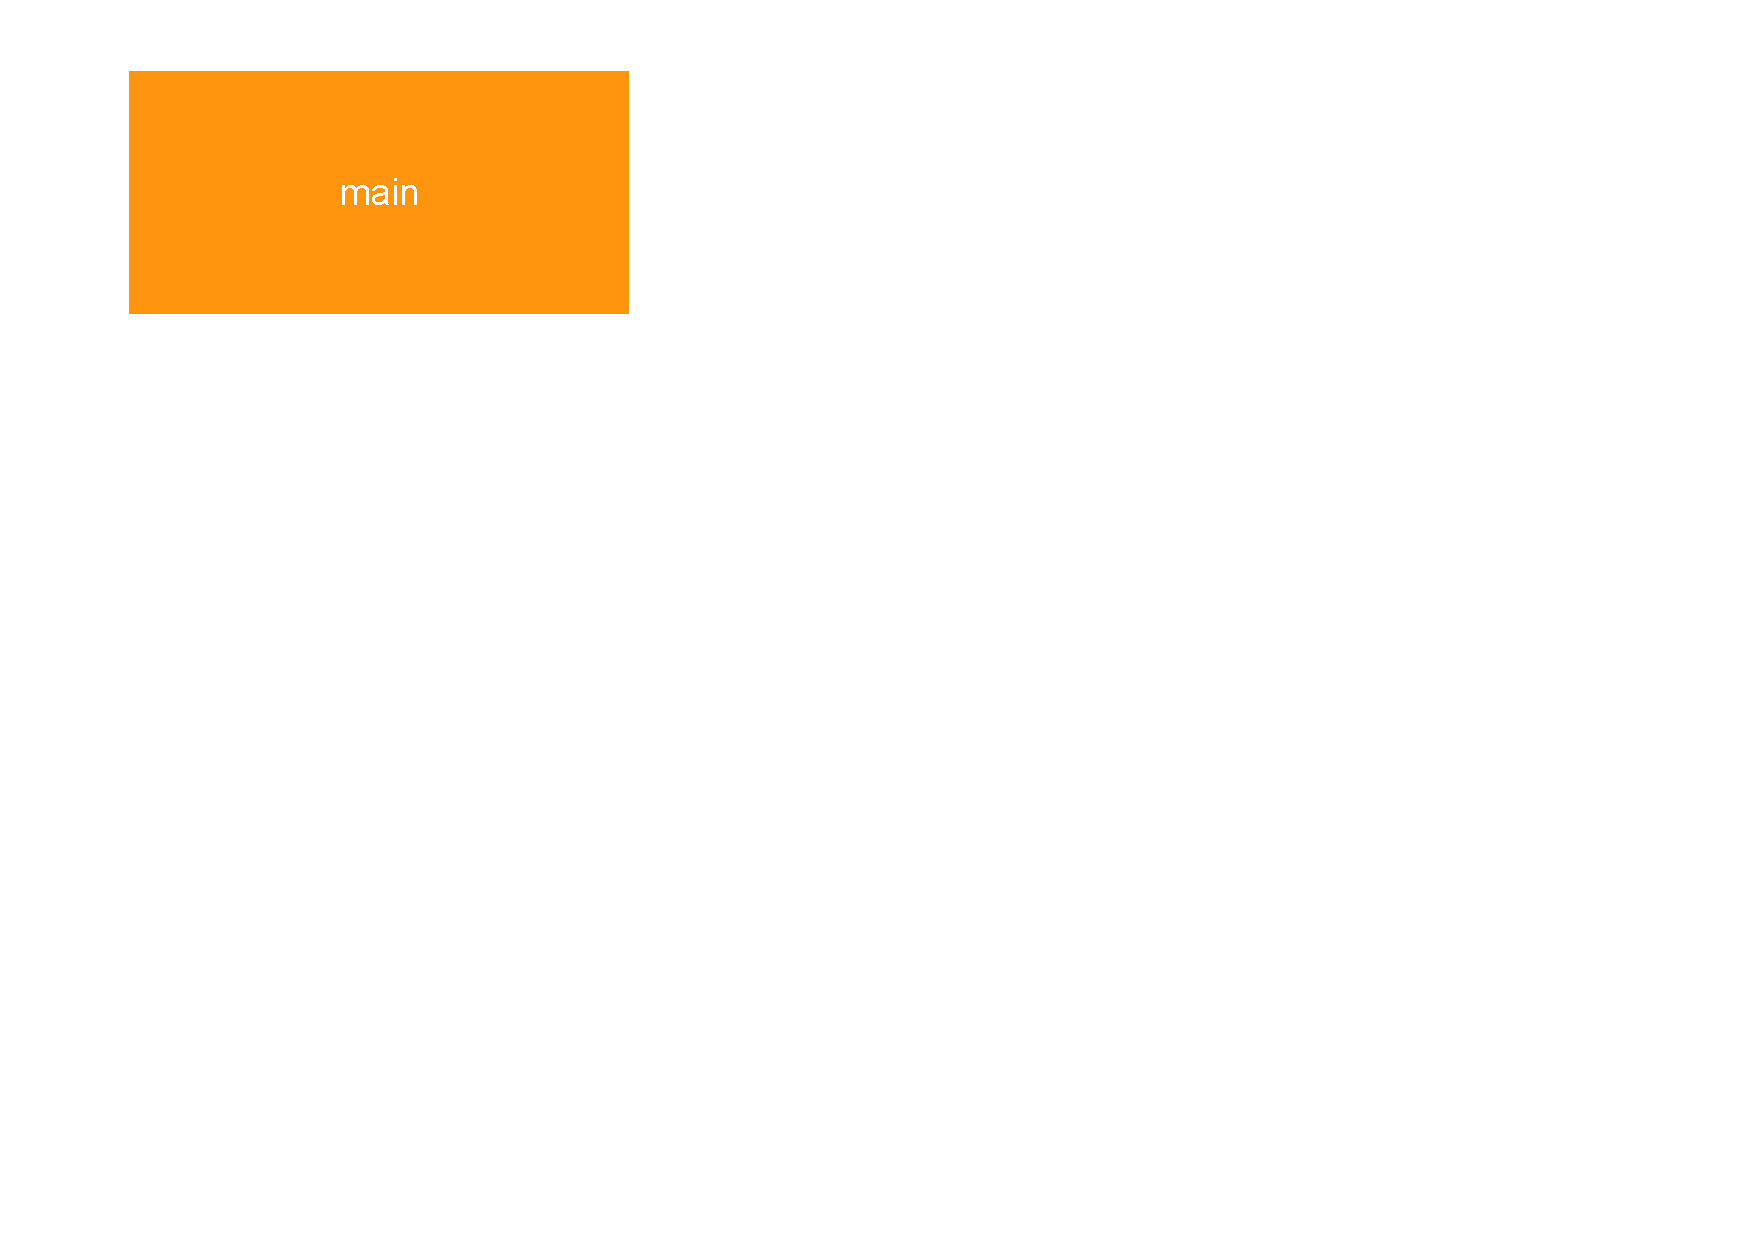
\includegraphics[scale=0.34]{include/multi1.pdf}}
    \only<2>{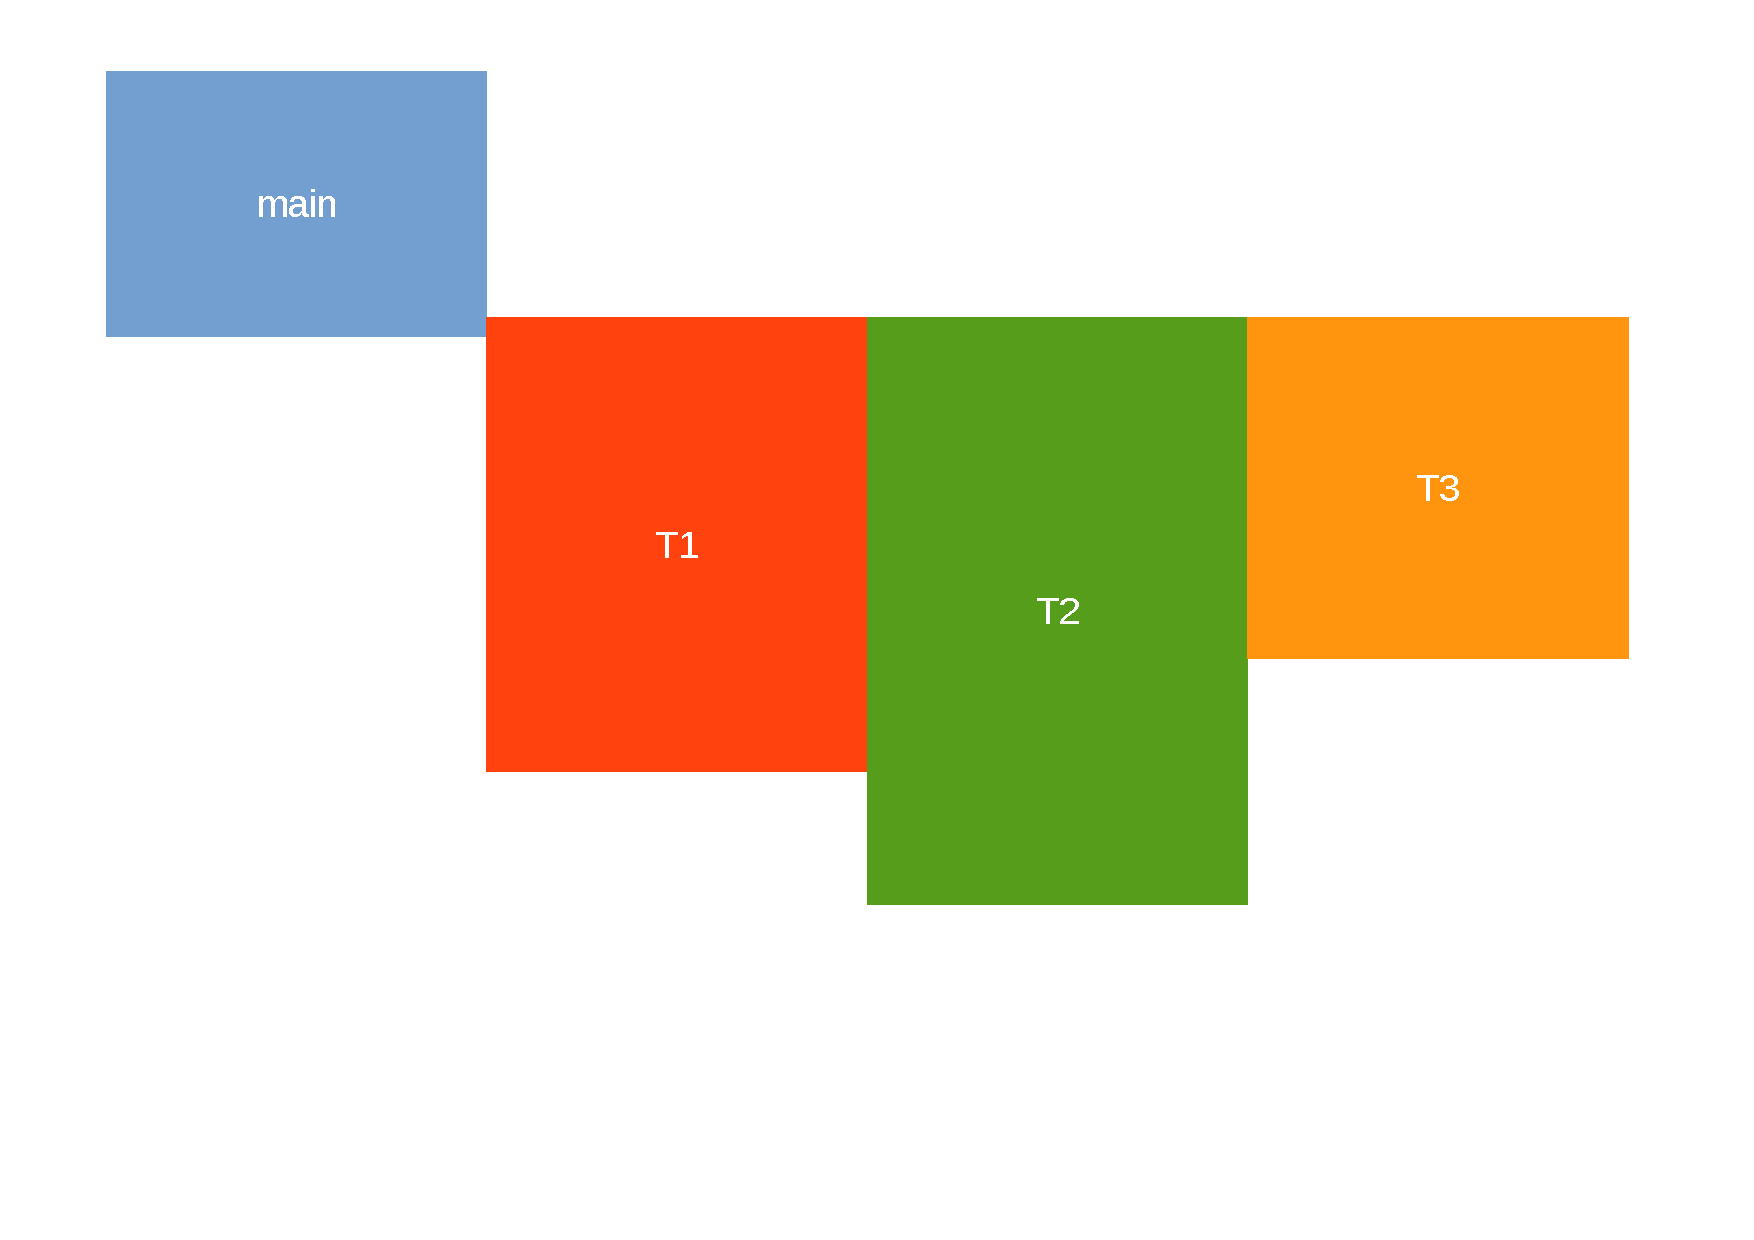
\includegraphics[scale=0.34]{include/multi2.pdf}}
    \only<3>{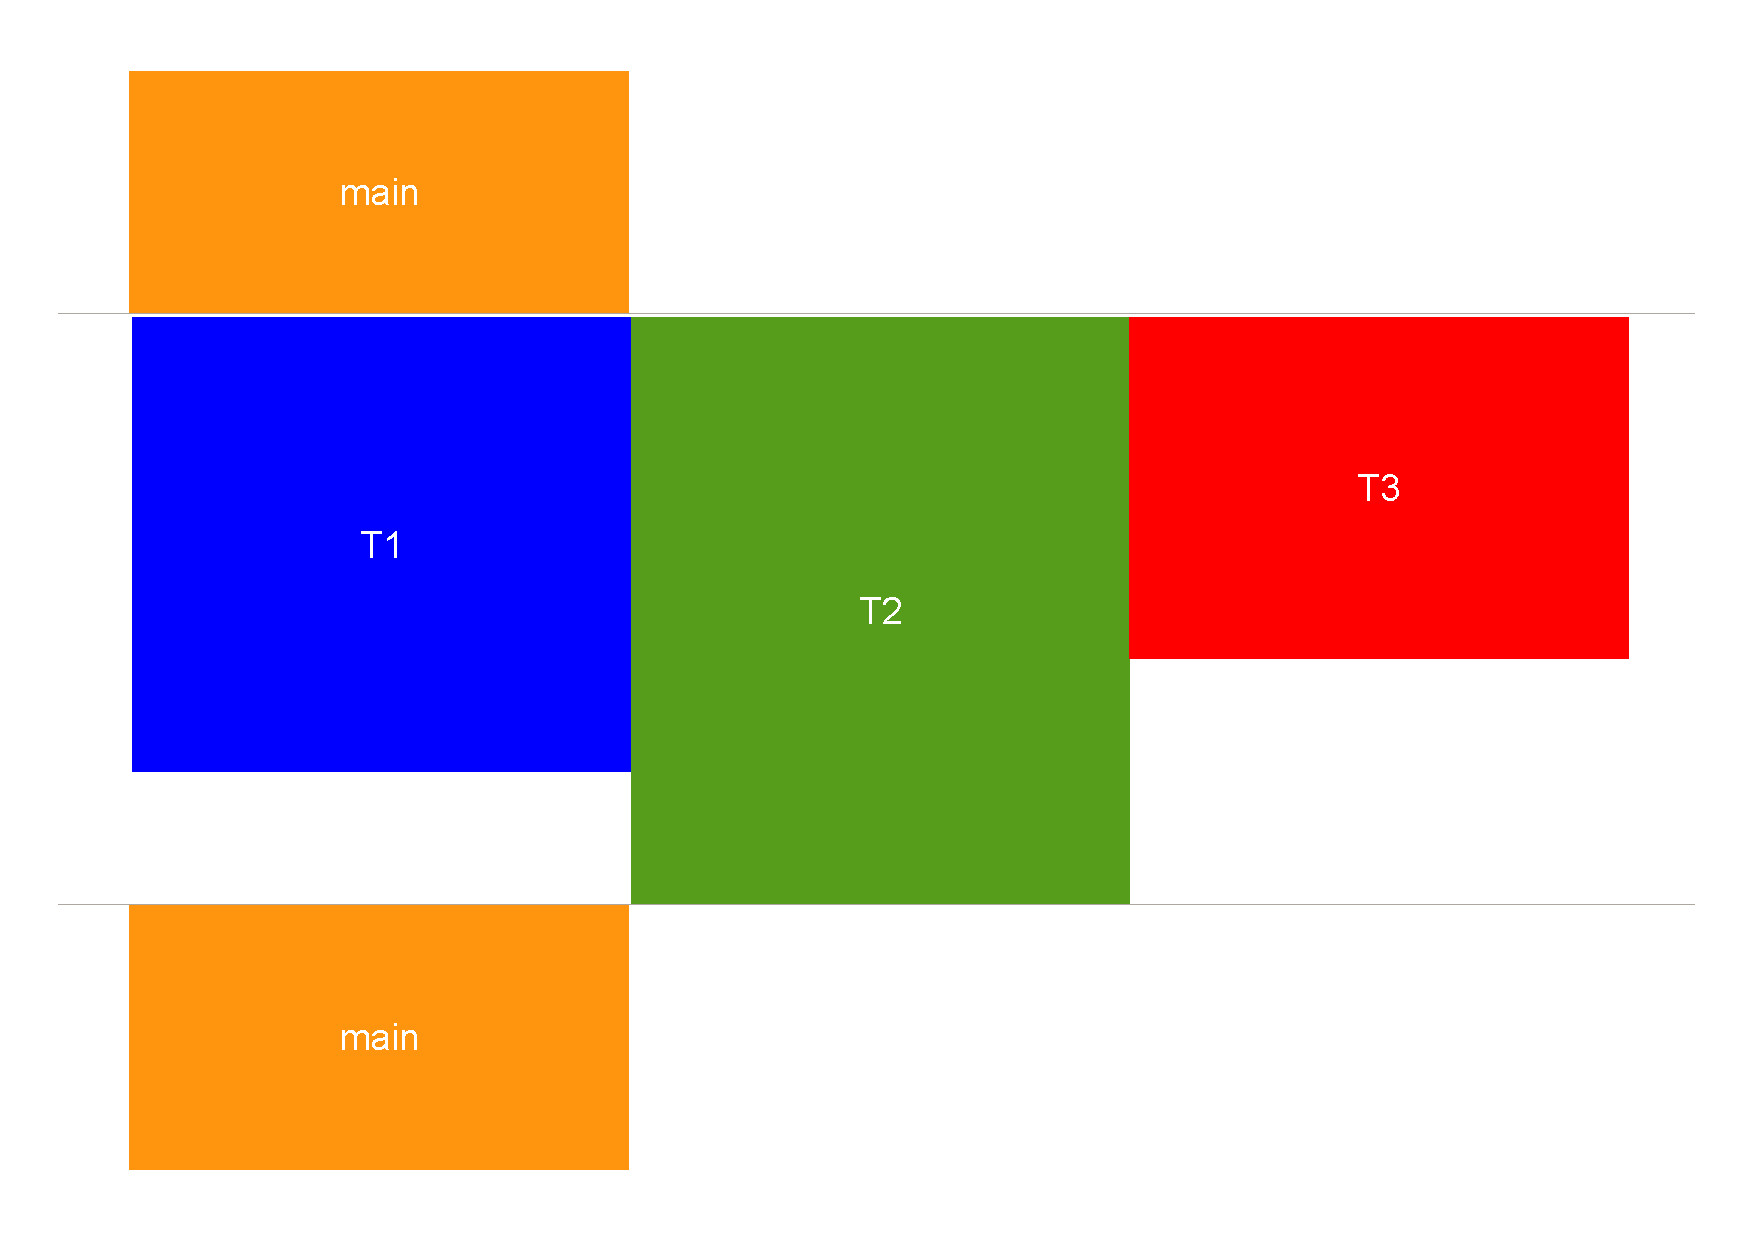
\includegraphics[scale=0.34]{include/multi3.pdf}}
  \end{center}

\end{frame}

% --------------------------------------------------

\begin{frame}
  \frametitle{Parallélisation de Routino}
  \framesubtitle{\'Evaluation - Utilisation CPU par tâche}
  
  \begin{center}
    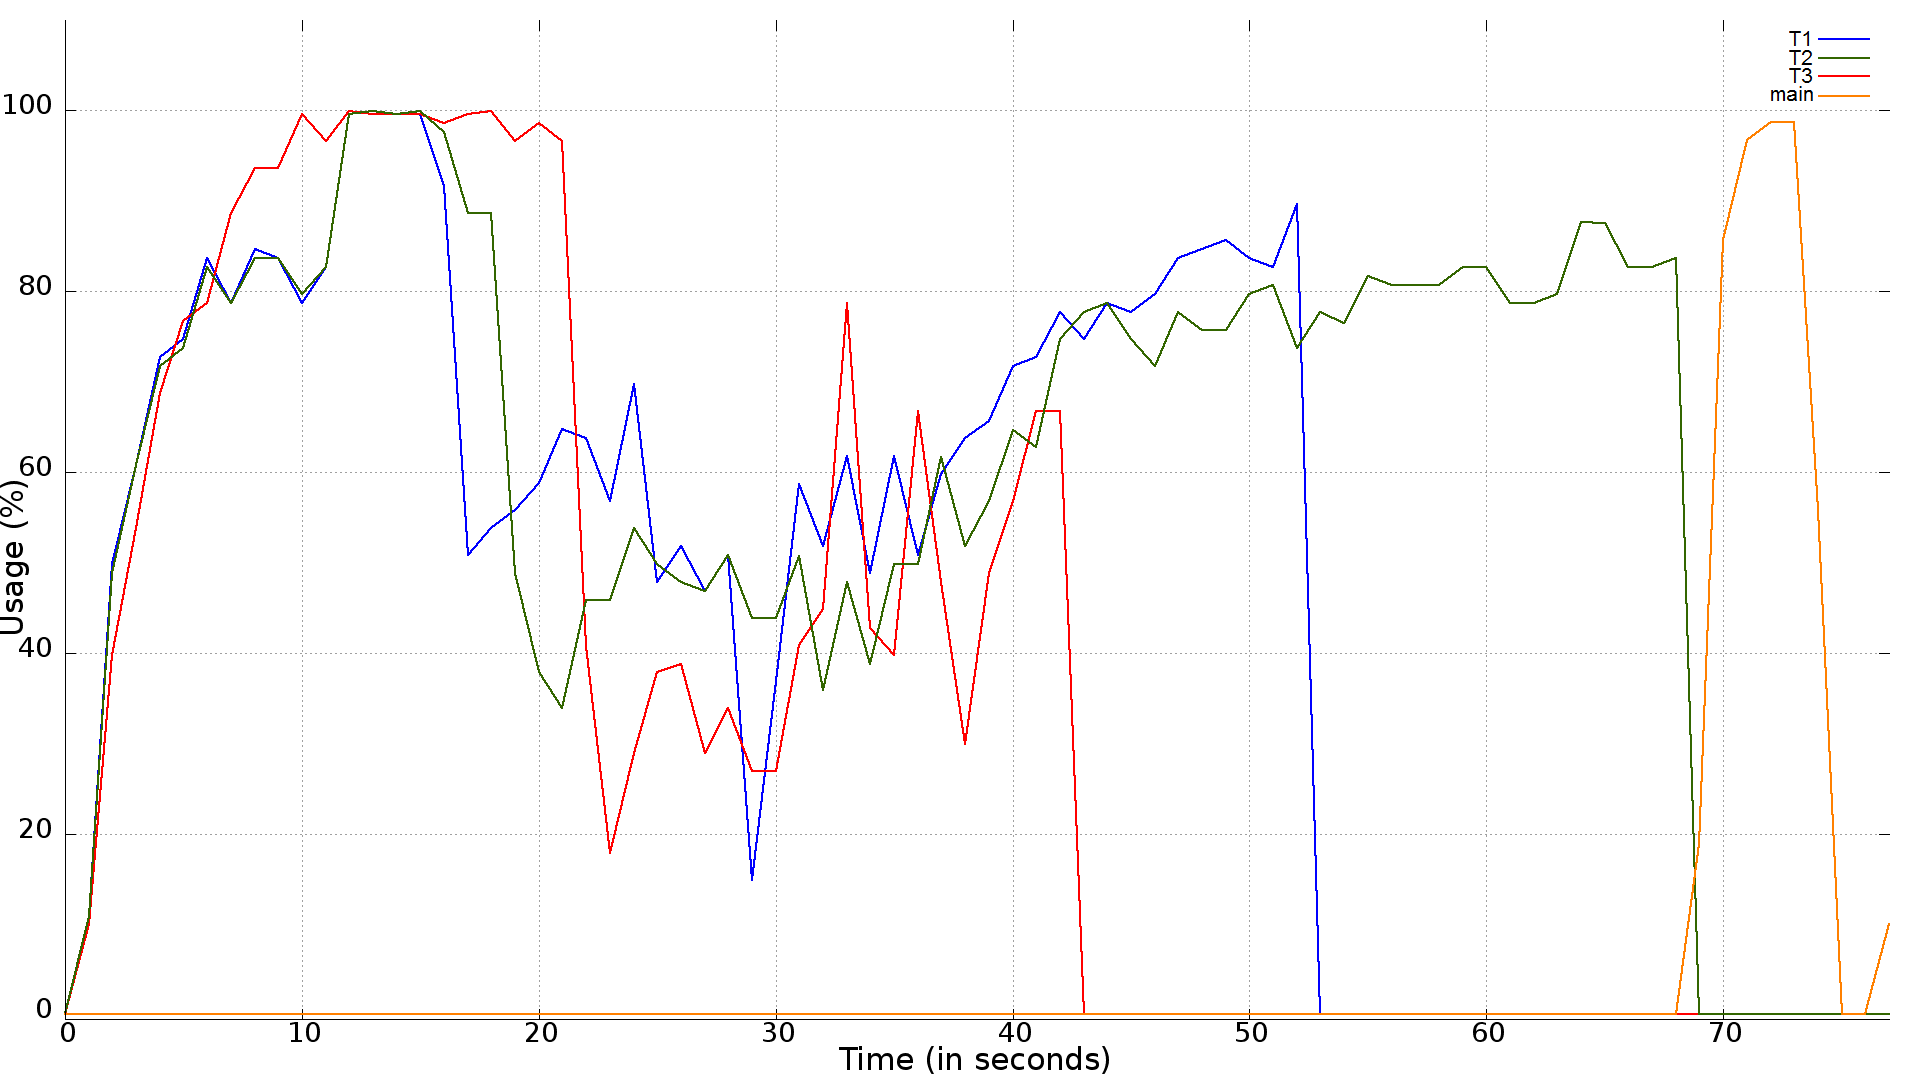
\includegraphics[scale=0.18]{include/thread_usage.png}
  \end{center}
  \visible<2>{
    \begin{exampleblock}{Observations}
      On note les terminaisons différées des tâches et la reprise du
      \texttt{main} après la barrière de synchronisation.
    \end{exampleblock}
  }
\end{frame}

% --------------------------------------------------

\begin{frame}
  \frametitle{Parallélisation de Routino}
  \framesubtitle{\'Evaluation - Gain de performance}

  \begin{center}
    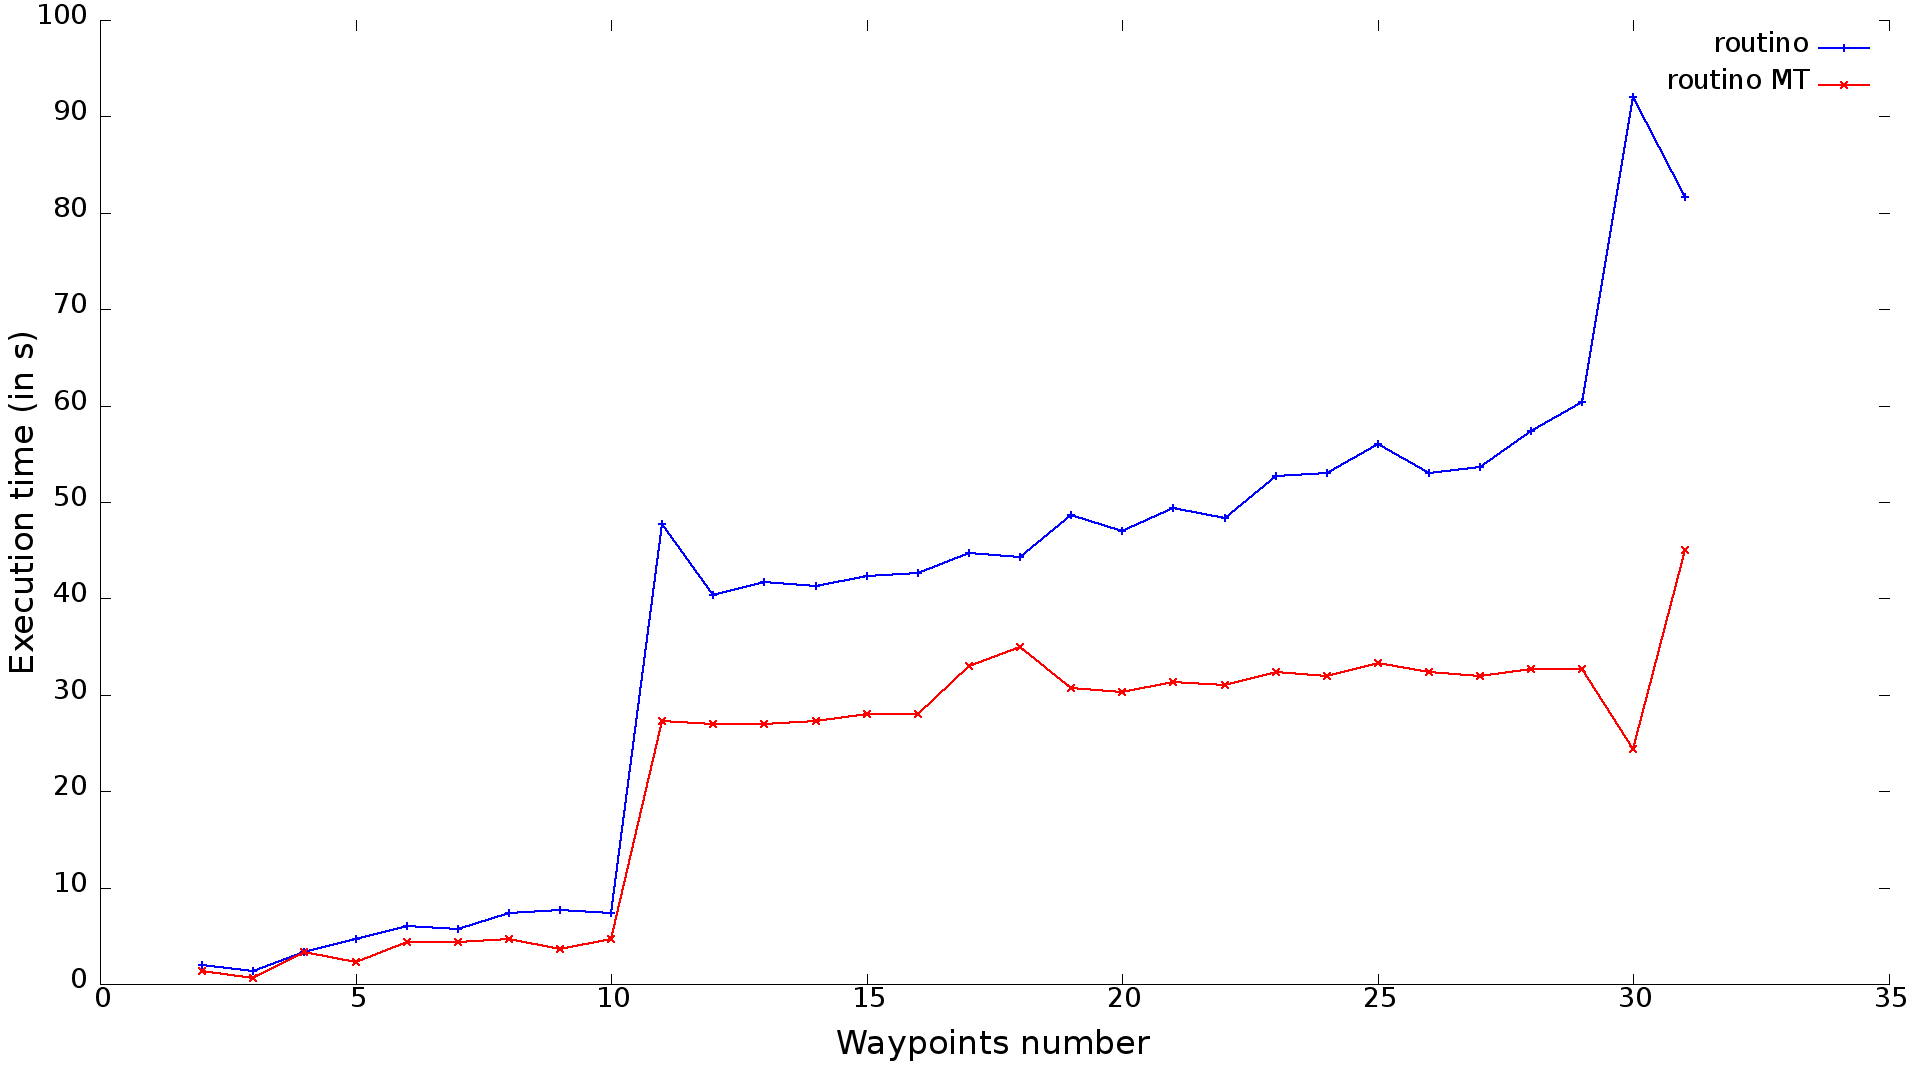
\includegraphics[scale=0.18]{include/speedup.png}
  \end{center}
  \visible<2>{
    \begin{exampleblock}{Observations}
      \begin{itemize}
        \item Temps divisé par 2 au mieux car plus de calculs par segment
        \item Les longs segments offrent un meilleur gain
      \end{itemize}
    \end{exampleblock}
  }
\end{frame}


%------------------------------------------------

\begin{frame}
  \frametitle{\'Etude d'impact sur une tâche temps-réel}
  \framesubtitle{Méthodologie}
  \begin{enumerate}
  \item<1-> Métriques
    \begin{itemize}
    \item Temps d'exécution
    \item Bande passante utilisée sur le système
    \end{itemize}
  \item<2-> Tâches temps-réel
    \begin{itemize}
    \item Benchmark MiBench
    \item Sous-ensemble d'applications représentatives d'un système automobile
    \end{itemize}
  \item<3-> Jeu de tests
    \begin{itemize}
    \item Tâche temps-réel en isolation
    \item Tâche temps-réel vs Routino (3 instances)
    \item Tâche temps-réel vs Routino MT (3 threads)
    \end{itemize}
  \item<4> Protocole
    \begin{itemize}
    \item[$T_0$] Lancement du/des Routino(s) si nécessaire (durée $\approx$
      45-80 s)
    \item[$T_0+\Delta$] Lancement de la tâche temps-réel (durée $<$ 100 ms)
    \end{itemize}
  \end{enumerate}
\end{frame}

%------------------------------------------------

\begin{frame}
  \frametitle{\'Etude d'impact sur une tâche temps-réel}
  \framesubtitle{Impact sur le temps d'exécution}
  \begin{center}
    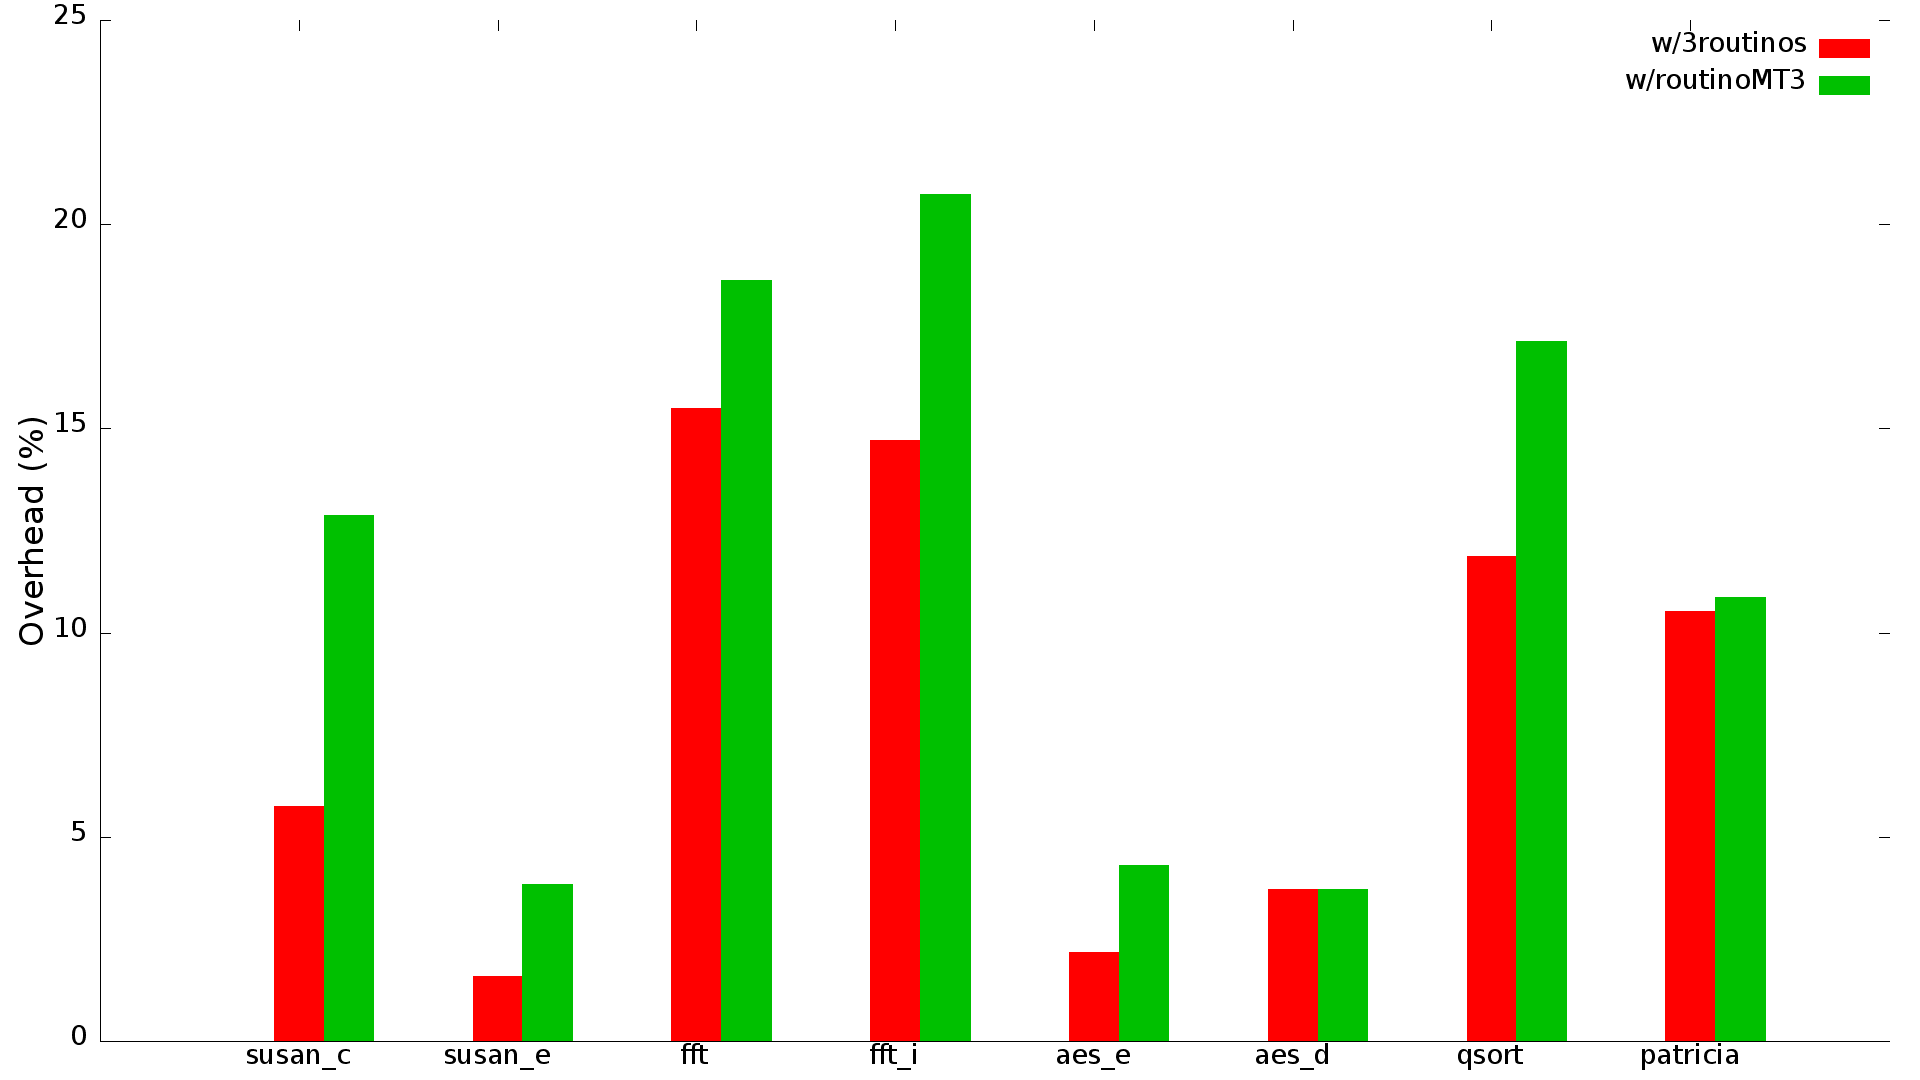
\includegraphics[scale=0.18]{include/overhead.png}
  \end{center}
  \visible<2>{
    \begin{exampleblock}{Observations}
      \begin{itemize}
      \item Augmentation de 2 à 20\% du temps d'exécution
      \item \'Ecart de surcoût non constant
      \end{itemize}
    \end{exampleblock}
  }
\end{frame}

%------------------------------------------------

\begin{frame}
  \frametitle{\'Etude d'impact sur une tâche temps-réel}
  \framesubtitle{Impact sur la bande passante}
  \begin{center}
    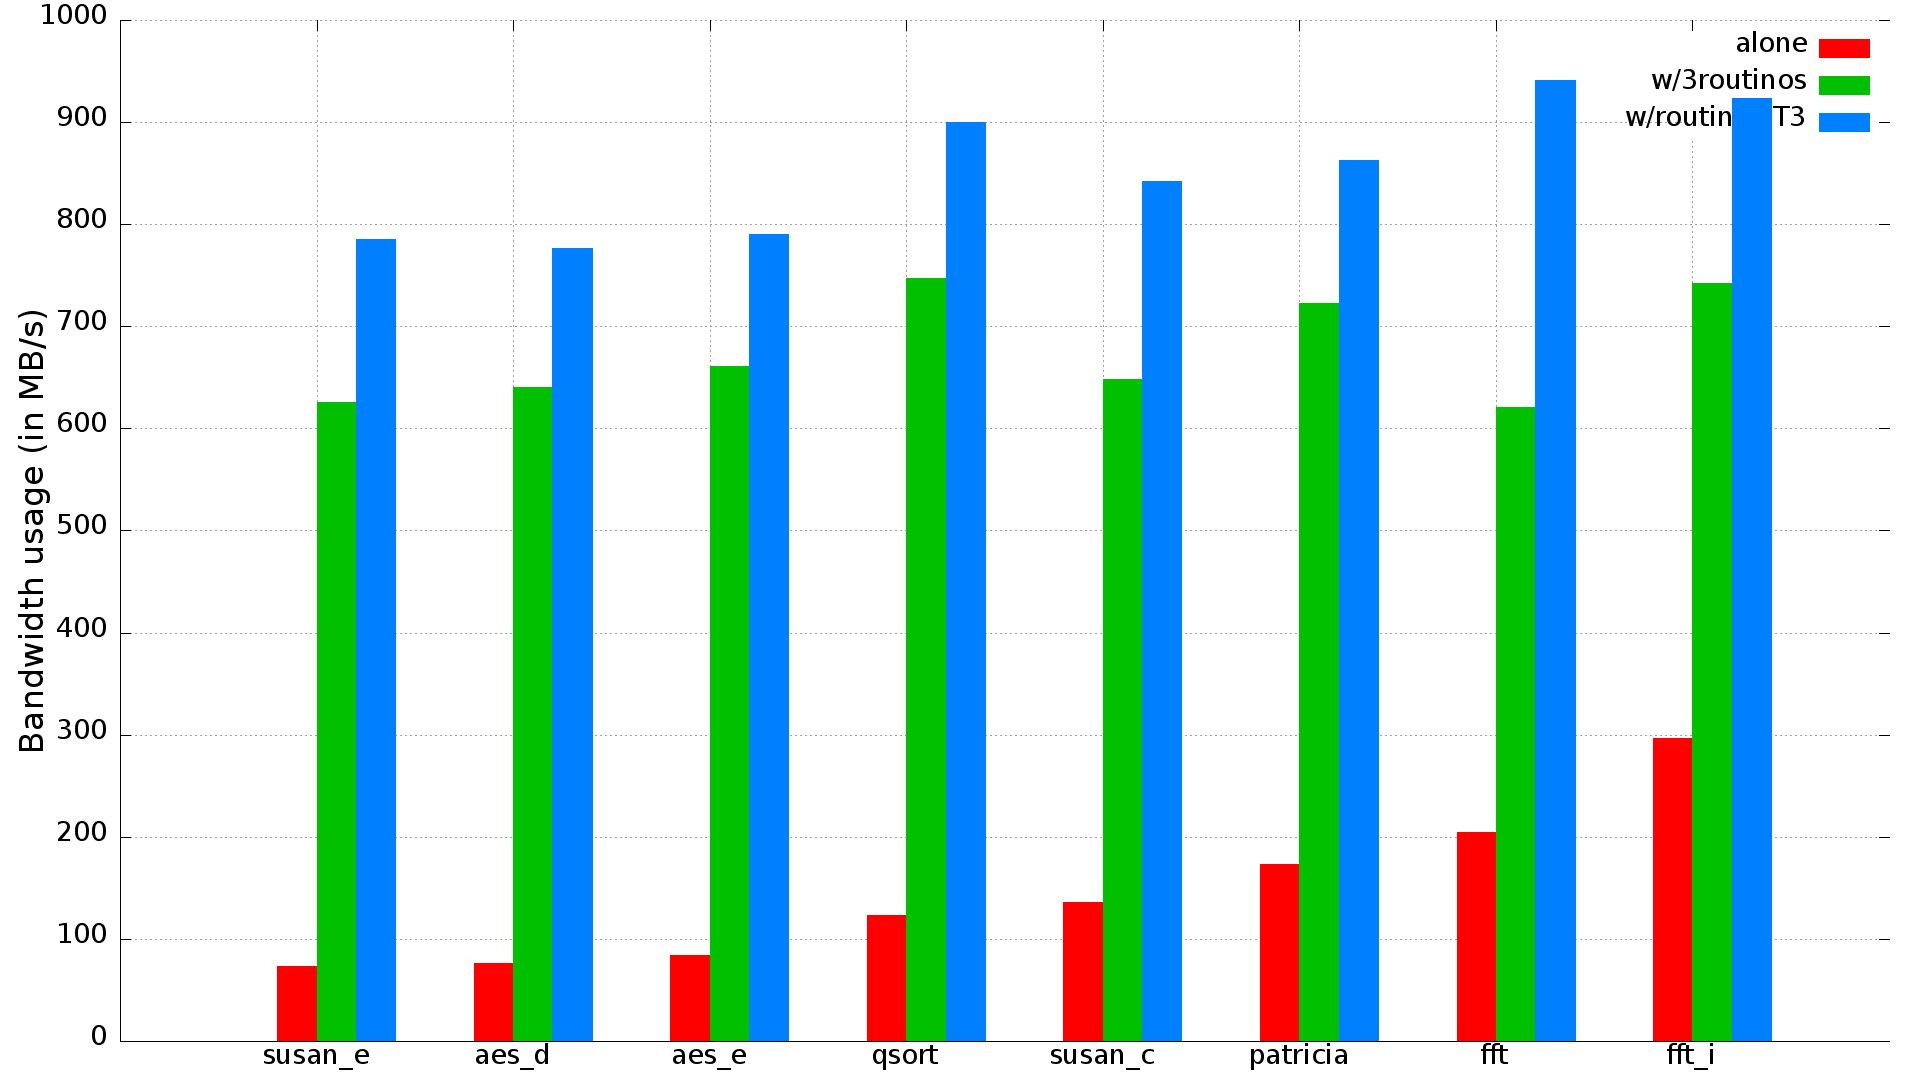
\includegraphics[scale=0.175]{include/bandwidth.png}
  \end{center}
  \visible<2>{
    \begin{exampleblock}{Observations}
      La bande passante utilisée est similaire pour toutes les tâches du 
      benchmark. Les différences sont notamment dûes aux durées d'exécution
      de chacune.
    \end{exampleblock}
  }
\end{frame}

%------------------------------------------------

\begin{frame}
  \frametitle{\'Etude d'impact sur une tâche temps-réel}
  \framesubtitle{Corrélation bande passante/overhead}
  \begin{center}
    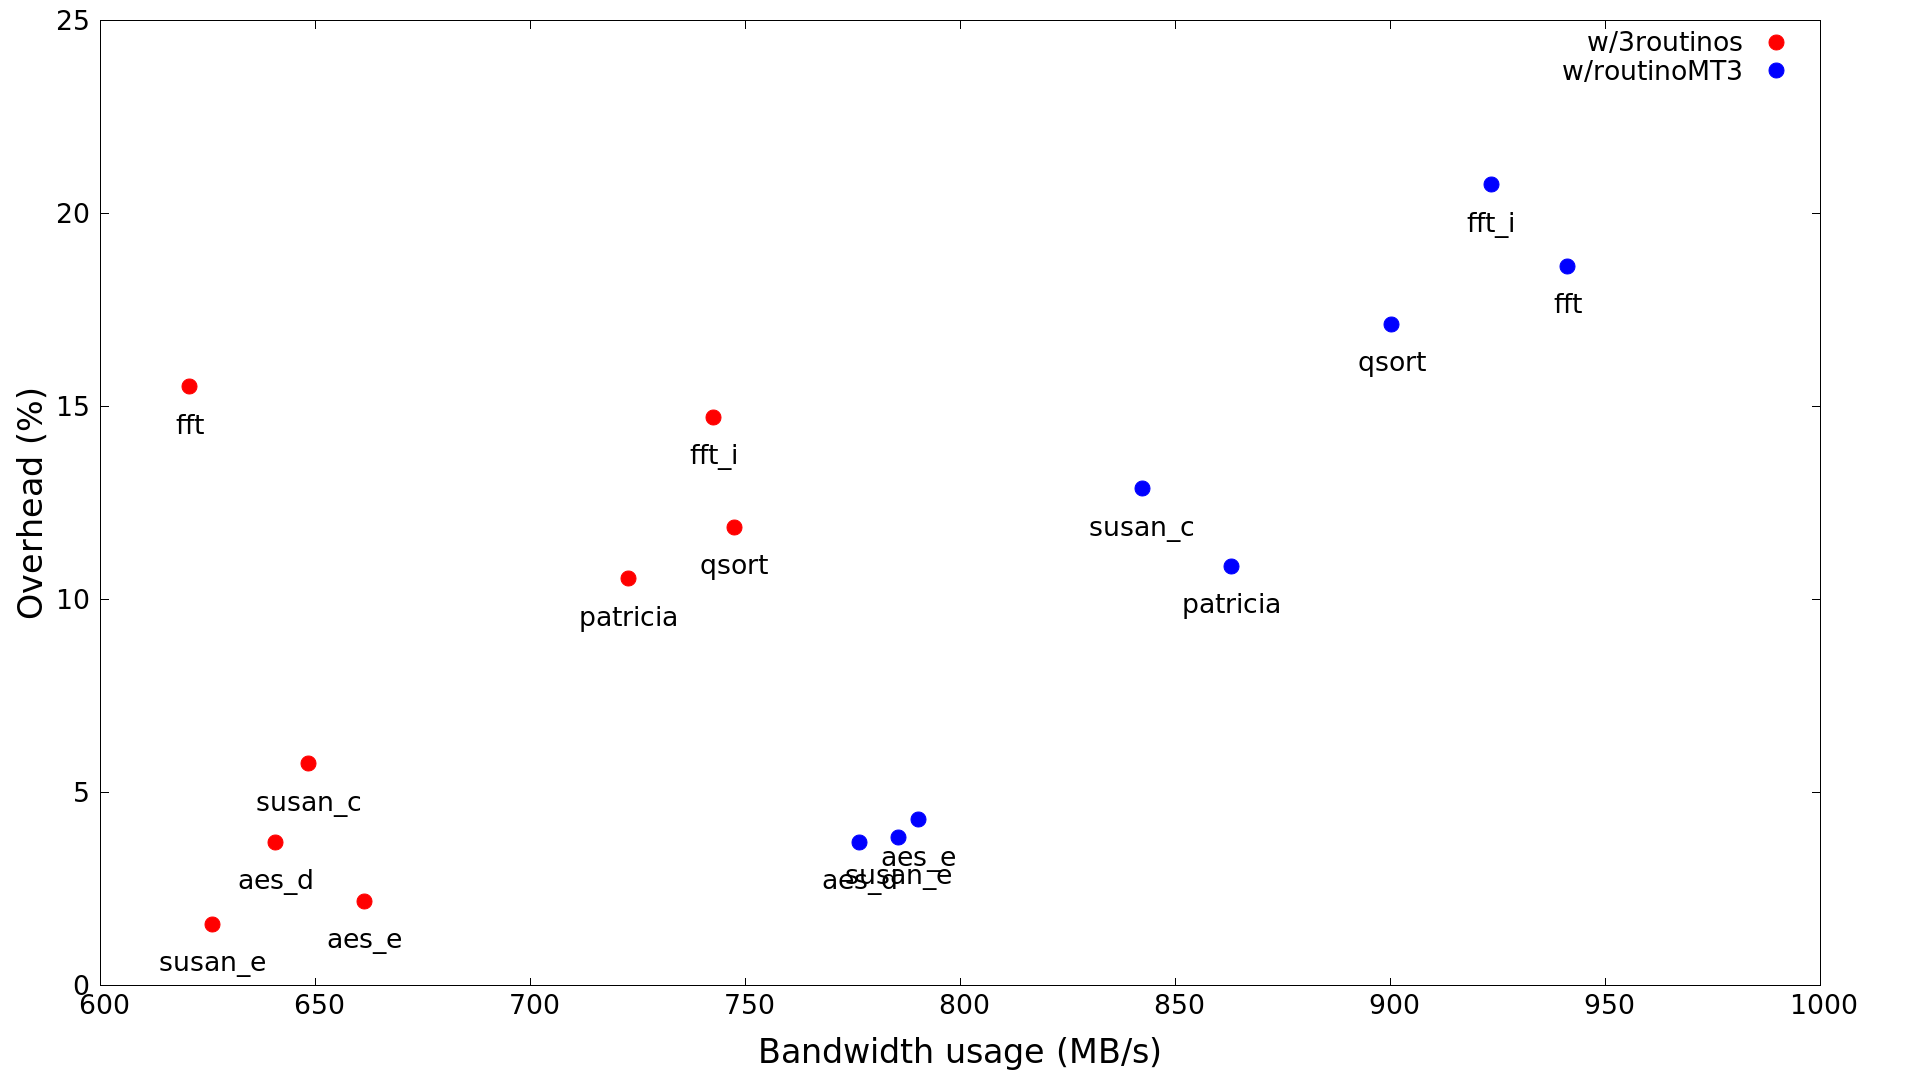
\includegraphics[scale=0.14]{include/correl.png}
  \end{center}
  \visible<2>{
    \begin{exampleblock}{Observation}
      Progression de l'overhead quasi-linéaire pour chaque type
      d'exécution (avec 3 instances de Routino ou avec RoutinoMT sur 3 threads)
    \end{exampleblock}
  }
\end{frame}

%------------------------------------------------

%---------------------------------------------------------------------------


%---------------------------------------------------------

\begin{frame}
\frametitle{Conclusion}
\begin{enumerate}
  \visible<1->{
  \item Réalisations
    \begin{itemize}
    \item Sélection d'une application
    \item Portage et parallélisation de l'application
    \item \'Etude de la parallélisation
    \item \'Etude de l'impact sur une tâche temps-réel MiBench
    \end{itemize}
  }
  \visible<2->{
  \item Travail à court terme
    \begin{itemize}
      \item Vérifier si l'overhead diminue avec l'algorithme d'ordonnancement
        d'Antoine Blin
      \item Soumettre un patch pour Routino
    \end{itemize}
  }
  \visible<3->{
    \item Travail à long terme
      \begin{itemize}
        \item \'Etendre la parallélisation aux trajets sans étapes
      \end{itemize}
  }
\end{enumerate}
\end{frame}

\end{document}
